\section{Experimental Evaluation}
\label{sec:evaluation}


We evaluate \Tool on the standard FPBench
benchmark suite~\cite{fpbench,fpbench-web} that uses the four basic operations we
currently support $\{+,-,\times,\div\}$.
%
Many of these benchmarks were also used in recent related work~\cite{probdaisy}
that we compare against.
%
The benchmarks come from a variety of domains: embedded software (\emph{bsplines}), linear classifications (\emph{classids}), physics computations (\emph{dopplers}), filters (\emph{filters}), controllers (\emph{traincars}, \emph{rigidBody}), polynomial approximations of functions (\emph{sine}, \emph{sqrt}), solving equations (\emph{solvecubic}), and global optimizations (\emph{trids}).
%
Since FPBench has been primarily used for worst-case roundoff error
analysis,  the benchmarks come with ranges for input variables, but they do not specify
input distributions.
%
We instantiate the benchmarks with three well-known distributions for all the
inputs: uniform, standard normal distribution,  and double exponential (\ie Laplace)
distribution with $\sigma=0.01$ which we will call `exp'. 
%
The normal and exp distributions get truncated to the given range.
%
We assume single-precision floating-point format for all
operands and operations, but it is straightforward to
extend \Tool to mixed-precision computations.


To assess the accuracy and performance of \Tool, we compare it with
PrAn~\cite{probdaisy}, the current state-of-the-art tool for automated analysis
of probabilistic roundoff errors.
%
PrAn currently supports only uniform and normal input distributions.
%
It offers six different tool configurations; for each benchmark, we run
all of them and report the best result.
%
We fix the number of intervals in each discretization to 50 to match PrAn.
%
We choose 99\% as the confidence interval for the computation of our conditional roundoff error (\cref{subsec:conderror}) and of PrAn's probabilistic error.
%d
We also compare our probabilistic error bounds against FPTaylor which performs worst-case roundoff error analysis, and hence it does not
take into account the distributions of the input variables.
%
We ran our experiments in parallel on a 4-socket 2.2 GHz 8-core Intel Xeon
E5-4620 machine with 128 GB of memory.

\newcolumntype{L}[1]{>{\raggedright\let\newline\\\arraybackslash\hspace{0pt}}m{#1}}

\begin{table*}[t!]
	\centering
	\scriptsize
	\caption{Roundoff error bounds reported by \Tool, PrAn, and FPTaylor given
	uniform (uni), normal (norm), and Laplace (exp) input distributions.
	We set the confidence interval to 99\% for \Tool and PrAn, and mark the smallest reported
	roundoff errors for each benchmark in bold. Asterisk (*) highlights a difference of more than one order of magnitude between \Tool and FPTaylor.}
\label{erroranalysis}
	\renewcommand{\arraystretch}{1.1}
	%\setlength{\tabcolsep}{0.3em} % for the horizontal padding
%		Benchmark & \Tool & Sampling & Golden & PrAn& \Tool & Sampling & Golden & FpTaylor\\
	\begin{tabular}{@{\extracolsep{2.3pt}}p{1.5cm}L{1.2cm}L{1.2cm}L{1.3cm}L{1.3cm}L{1.3cm}L{1.3cm}L{1.3cm}@{}}
		\toprule
		\multirow{4}{*}{Benchmark} & \multicolumn{2}{c}{uniform} & \multicolumn{2}{c}{normal} & \multicolumn{1}{c}{exp} &\multirow{4}{1.2cm}{FpTaylor}\\
		\cmidrule{2-3} \cmidrule{4-5} \cmidrule{6-6}
		& \multicolumn{1}{c}{\Tool} & \multicolumn{1}{c}{PrAn} & \multicolumn{1}{c}{\Tool} & \multicolumn{1}{c}{PrAn} & \multicolumn{1}{c}{\Tool} \\
		\midrule
		%bspline0 & 0.000000057135674709 & 6.114890618137056e-08 & 0.000000057135674709 & 6.114890618137056e-08 & 0.0000000571356747099591235019055996 &5.723754e-08 \\
		bspline0 & \textbf{5.71e-08} & 6.12e-08 & \textbf{5.71e-08} & 6.12e-08 & \textbf{5.71e-08} &5.72e-08 \\
		\mydashline{}
		%bspline1 & 0.00000018642444703231 & 2.0791491997727016e-07 & 0.000000186424447 & 2.0791491997727016e-07 & &0.000000069538953116 1.926176e-07 \\
		bspline1 & \textbf{1.86e-07} & 2.08e-07 & \textbf{1.86e-07} & 2.08e-07 & \textbf{6.95e-08} &1.93e-07 \\
		\mydashline{}
		%bspline2 & 0.00000019395263 & 2.12482123801886354e-07 & 0.00000019395263739 & 2.12482123801886354e-07 & 0.00000002112086 & 2.100581e-07 \\
		bspline2 & \textbf{1.94e-07} & 2.13e-07 & \textbf{1.94e-07} & 2.13e-07 & \textbf{2.11e-08} &2.10e-07 \\
		\mydashline{}
		%bspline3 & 0.0000000422199574 & 4.654427574900906e-08 & 0.0000000422199574 & 4.654427574900906e-08 & 0.000000000007620570 & 4.221996e-08 \\
		bspline3 & \textbf{4.22e-08} & 4.65e-08 & \textbf{4.22e-08} & 4.65e-08 & \textbf{7.62e-12}* &4.22e-08 \\
		\mydashline{}
		%classids0 & 0.000006925939821221243464 & 8.64562812674436851e-06 & 0.00000334549928 & 8.638177546147444e-06 & 0.000001701560 & 6.850891e-06 \\
		classids0 & \textbf{6.93e-06} & 8.65e-06 & \textbf{4.45e-06} & 8.64e-06 & \textbf{1.70e-06} &6.85e-06 \\
		\mydashline{}
		%classids1 & 0.00000370535418918 & 4.6280713745928506e-06 & 0.0000026816110 & 4.624346084294389e-06 & 0.0000007622609 & 3.618862e-06 \\
		classids1 & \textbf{3.71e-06} & 4.63e-06 & \textbf{2.68e-06} & 4.62e-06 & \textbf{7.62e-07} &3.62e-06 \\
		\mydashline{}
		%classids2 & 0.000005227841 & 7.3150730487993595e-06 & 0.000003852640 & 7.3150730487993595e-06 & 0.0000014554841 & 5.154284e-06 \\
		classids2 & \textbf{5.23e-06} & 7.32e-06 & \textbf{3.85e-06} & 7.32e-06 & \textbf{1.46e-06} &5.15e-06 \\
		\mydashline{}
		%doppler1 & 0.00007952656 & 0.00011734932800403605 & 0.000000507835236650 & 0.00011734932800403605 & 0.0000004870285655 &6.101980e-05 \\
		doppler1 & \textbf{7.95e-05} & 1.17e-04 & \textbf{5.08e-07}* & 1.17e-04 & \textbf{4.87e-07}* &6.10e-05 \\
		\mydashline{}
		%doppler2 & 0.00014261120785 & 0.0002454344786446796 & 0.00000066062146370 & 0.0002454344786446796 & 0.00000062800023189 &1.110593e-4 \\
		doppler2 & \textbf{1.43e-04} & 2.45e-04 & \textbf{6.61e-07}* & 2.45e-04 & \textbf{6.28e-07}* &1.11e-04 \\
		\mydashline{}
		%doppler3 & 0.0000455140 & 5.1226582087069294e-05 & 0.000000911339546 & 5.1226582087069294e-05 & 0.000000894817972 & 3.409578e-5 \\
		doppler3 & \textbf{4.55e-05} & 5.12e-05 & \textbf{9.11e-07}* & 5.12e-05 & \textbf{8.95e-07}* &3.41e-05 \\
		\mydashline{}
		%example & 0.000017642975080 & 1.7166137922686175e-05 & 0.000001435459353160 & 1.69617791405991218e-05 & 0.0000003339084742037 &1.764298e-5 \\
		%example & 1.76e-05 & 1.72e-05 & \textbf{1.44e-06} & 1.69e-05 & 3.3e-07 &1.76e-05 \\
		%\mydashline{}		
		%filter1 & 0.0000001251697548720 & 2.02655795789041802e-07 & 0.0000001251697 & 2.02655795789041802e-07 & 0.0000000054249540 & 1.251698e-07 \\
		filter1 & \textbf{1.25e-07} & 2.03e-07 & \textbf{1.25e-07} & 2.03e-07 & \textbf{5.43e-09}* &1.25e-07 \\
		\mydashline{}
		%filter2 & 0.00000079282326 & 1.00646702948990574e-06 & 0.0000006125518145 & 1.00646702948990574e-06 & 0.000000029028233376 & 7.930026e-07 \\
		filter2 & \textbf{7.93e-07} & 1.01e-06 & \textbf{6.13e-07} & 1.01e-06 & \textbf{2.90e-08}* &7.93e-07 \\
		\mydashline{}
		%filter3 & 0.000002342142453 & 2.85808266958062087e-0 & 0.000002048730 & 2.86920886993869378e-06 & 0.00000010851954 & 2.227247e-06 \\
		filter3 & \textbf{2.34e-06} & 2.86e-06 & \textbf{2.05e-06} & 2.87e-06 & \textbf{1.09e-07}* &2.23e-06 \\
		\mydashline{}
		%filter4 & 0.000004150741 & 5.19976694470474714e-06 & 0.0000056311846761 & 5.19976696266371479e-06 & 0.00000046124223 & 3.812784e-06 \\
		filter4 & \textbf{4.15e-06} & 5.20e-06 & \textbf{4.15e-06} & 5.20e-06 & \textbf{4.61e-07} &3.81e-06 \\
		\mydashline{}
		%rigidbody1 & 0.0001735687 & 0.00015830993720555853 & 0.000006137299 & 0.00015830993720555853 & 0.00000047992216 & 1.583099e-04 \\
		rigidbody1 & 1.74e-04 & \textbf{1.58e-04} & \textbf{6.14e-06}* & 1.58e-04 & \textbf{4.80e-07}* &1.58e-04 \\
		\mydashline{}
		%rigidbody2 & 0.0195775037232124424 & 9.69744108465421647e-03 & 0.0000598889960 & 9.69744108465421647e-03 & 0.00000095487503524 & 1.936293e-02 \\
		rigidbody2 & 1.96e-02 & \textbf{9.70e-03} & \textbf{5.99e-05}* & 9.70e-03 & \textbf{9.55e-07}* & 1.94e-02 \\
		\mydashline{}
		%sine & 0.0000002367187461 & 2.3953816138538605e-07 & 0.0000002367187461 & 2.3953816138538605e-07 & 0.0000000149042919777273723504 & 2.378573e-07 \\
		sine & \textbf{2.37e-07} & 2.40e-07 & \textbf{2.37e-07} & 2.40e-07 & \textbf{1.49e-08}* &2.38e-07 \\
		%\mydashline{}
		%sineorder3 & 0 & 4.05824589484735543e-07 & 0 & 4.05824589448069794e-07 & 3.286717e-07 \\
		%sineorder3 & 0 & 4.06e-07 & 0 & 4.06e-07 & 3.29e-07 \\
		\mydashline{}
		%solvecubic & 0.00001780083107 & 1.8340570336392748e-05 & 0.00000683768382145 & 1.8340570336392748e-05 & 0.000002761309051240668 & 1.603518e-05 \\
		solvecubic & \textbf{1.78e-05} & 1.83e-05 & \textbf{6.84e-06} & 1.83e-05 & \textbf{2.76e-06} & 1.60e-05 \\
		\mydashline{}
		%sqrt & 0.0001539099116173 & 1.54254744252888847e-04 & 0.0000011027971519376123 & 1.54254744252888847e-04 & 0.000000246062237188127055 & 1.511672e-04 \\
		sqrt & \textbf{1.54e-04} & \textbf{1.54e-04} & \textbf{1.10e-06}* & 1.54e-04 & \textbf{2.46e-07}* &1.51e-04 \\
		\mydashline{}
		%traincars1 & 0.00175989103116780849466171264648437500000000000002 & 1.95728428775231198e-03 & 0.00082550 & 1.95728428775231198e-03 & 0.000450416840 & 1.741275e-03 \\
		traincars1 & \textbf{1.76e-03} & 1.96e-03 & \textbf{8.26e-04} & 1.96e-03 & \textbf{4.50e-04} &1.74e-03 \\
		\mydashline{}
		%traincars2 & 0.0010428651220 & 1.32745391717492829e-03 & 0.0003610321 & 1.32745391717492829e-03 & 0.00002833656 & 9.459025e-04 \\
		traincars2 & \textbf{1.04e-03} & 1.36e-03 & \textbf{3.61e-04} & 1.36e-03 & \textbf{2.83e-05}* &9.46e-04 \\
		\mydashline{}
		%traincars3 & 0.017522481703072 & 2.29215064351089908e-02 & 0.00956279 & 2.29215064351089908e-02 & 0.0008950481065 & 1.795588e-02 \\
		traincars3 & \textbf{1.75e-02} & 2.29e-02 & \textbf{9.56e-03} & 2.29e-02 & \textbf{8.95e-04}* &1.80e-02 \\
		\mydashline{}
		%traincars4 & 0.181406716226774 & 2.29869604459963739e-01 & 0.0886905587 & 2.29869604459963739e-01 & 0.0073290 & 1.814067e-01 \\
		traincars4 & \textbf{1.81e-01} & 2.30e-01 & \textbf{8.87e-02} & 2.30e-01 & \textbf{7.33e-03}* &1.81e-01 \\
		\mydashline{}
		%trid1 & 6.01e-03 & 0.006027221781550907 & 0.000015763566 & 0.006027221781550907 & 0.000015760772 & 6.059647e-3 \\
		trid1 & \textbf{6.01e-03} & 6.03e-03 & \textbf{1.58e-05}* & 6.03e-03 & \textbf{1.58e-05}* &6.06e-03 \\
		\mydashline{}
		%trid2 & 0.010246651681654 & 1.16831463189252341e-02 & 2.42e-05 & 1.16831463189252341e-02 & 0.0000242665417 & 1.031161e-2 \\
		trid2 & \textbf{1.03e-02} & 1.17e-02 & \textbf{2.42e-05}* & 1.17e-02 & \textbf{2.43e-05}* &1.03e-02 \\
		\mydashline{}
		%trid3 & 0.0174517932318 & 1.94854738656431436e-02 & 0.00006794929612397 & 1.94854738656431436e-02 & 0.000067710877 & 1.746798e-2 \\
		trid3 & \textbf{1.75e-02} & 1.95e-02 & \textbf{6.80e-05}* & 1.95e-02 & \textbf{6.77e-05}* &1.75e-02 \\
		\mydashline{}
		%trid4 & 0.0269317630445584 & 2.88391116337152197e-02 & 0.0002641677870 & 3.03344729618402197e-02 & 0.000264167787 & 2.660800e-2 \\
		trid4 & \textbf{2.69e-02} & 2.88e-02 & \textbf{2.64e-04}*& 3.03e-02 & \textbf{2.64e-04}* & 2.66e-02 \\
		\bottomrule
	\end{tabular}
\end{table*}




Table~\ref{erroranalysis} compares roundoff errors reported by \Tool, PrAn, and
FPTaylor.
%
\Tool outperforms PrAn by computing tighter probabilistic error bounds on
almost all benchmarks, occasionally by orders of magnitude.
%
In the case of uniform input distributions, \Tool provides tighter bounds for
20 out of 27 benchmarks, for 6 benchmarks the bounds from PrAn are tighter,
while for \emph{sqrt} they are the same.
%
In the case of normal input distributions, \Tool provides tighter bounds for 26
out of 27 benchmarks, while for \emph{bspline3} the bounds from PrAn are
tighter.
%
%We provide a likely explanation for this in \cref{sec:related-work}.
%
Unlike PrAn, \Tool supports probabilistic output range analysis as well.
%
Table~\ref{rangeanalysis} in \cref{sec:appdx-evaluation} presents detailed
range analysis results.
%, which we do not discuss in detail due to lack of space.


In Table~\ref{erroranalysis}, of particular interest are benchmarks (6 for
normal and 10 for exp) where the error bounds generated by \Tool for the 99\%
confidence interval are at least an order of magnitude tighter than the
worst-case bounds generated by FPTaylor.
%
For such a benchmark and input distribution, \Tool's results inform a user that
there is an opportunity to optimize the benchmark (e.g., by reducing precision
of floating-point operations) if their use-case can handle at most 1\% of
inputs generating roundoff errors that exceed a user-provided bound.
%
FPTaylor's results, on the other hand, do not allow for a user to explore such
fine-grained trade-offs since they are worst-case and do not take probabilities
into account.

\begin{figure}[tb]
	\centering
	\begin{tabular}{l l}
		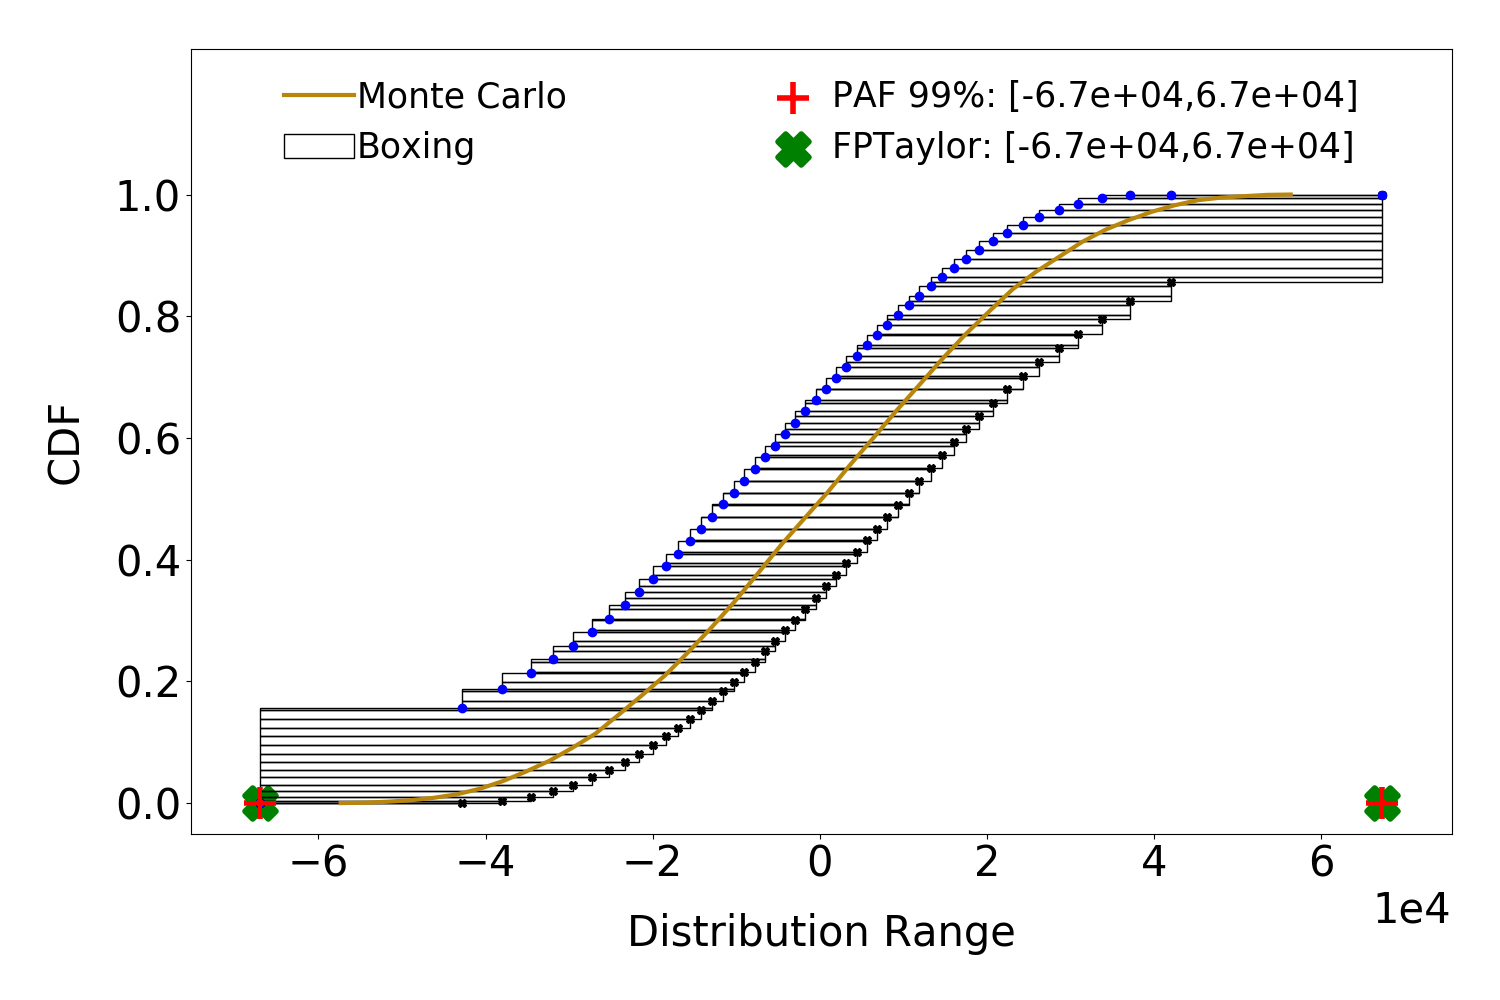
\includegraphics[width=0.5\textwidth]{pics/traincars3_range_CDF.png}
		&
		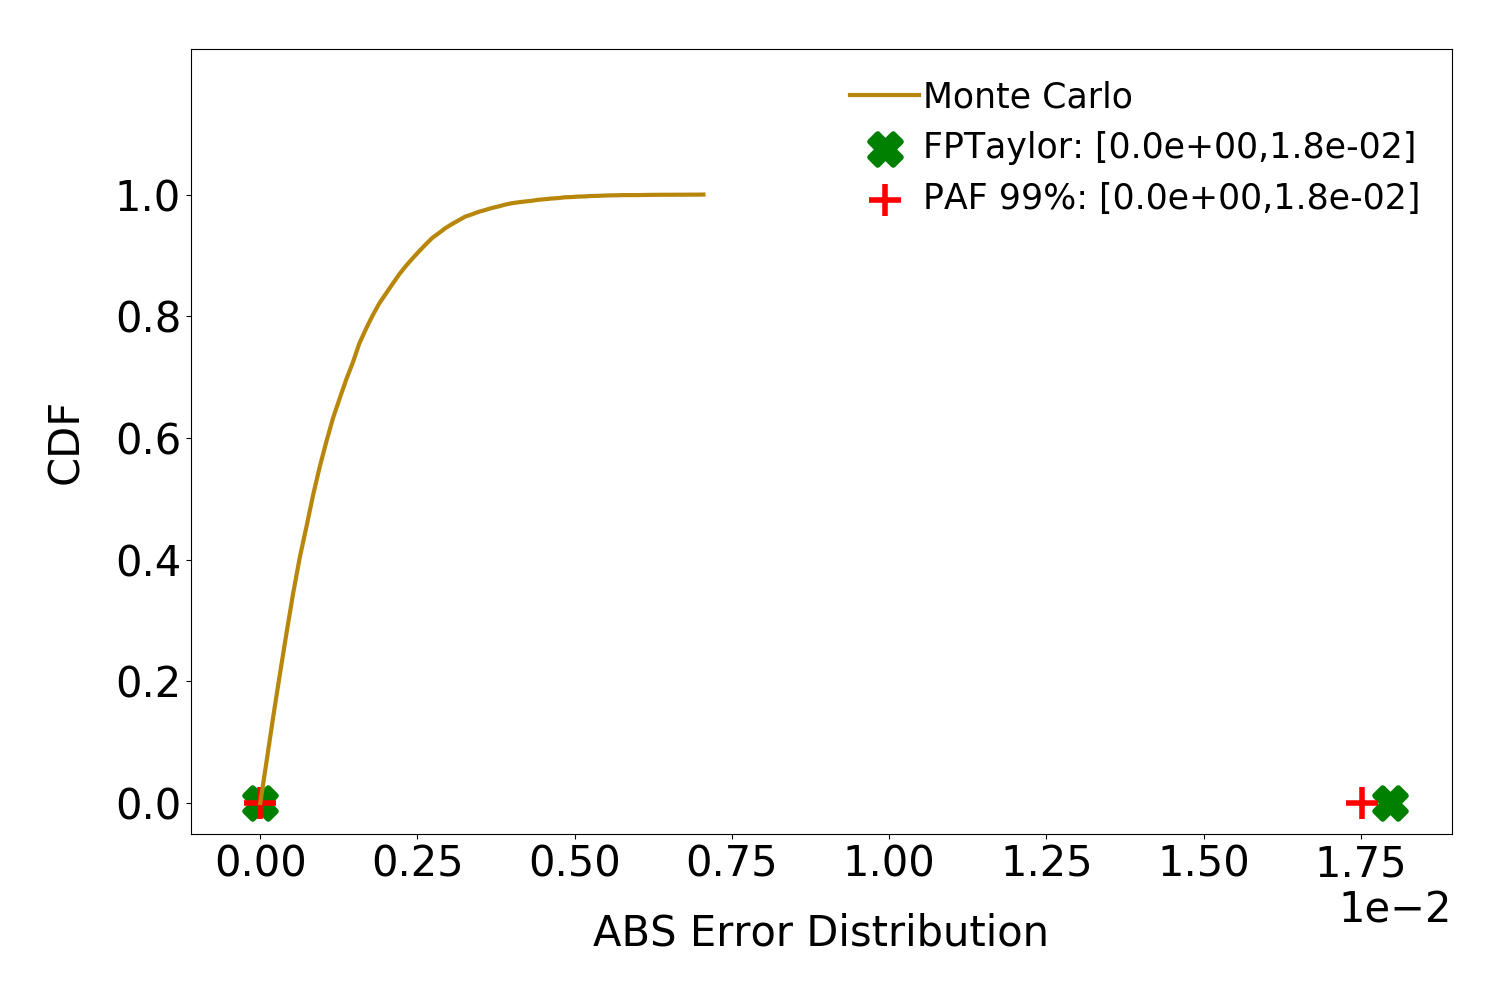
\includegraphics[width=0.5\textwidth]{pics/traincars3_abs_error_CDF.png}
		\\
		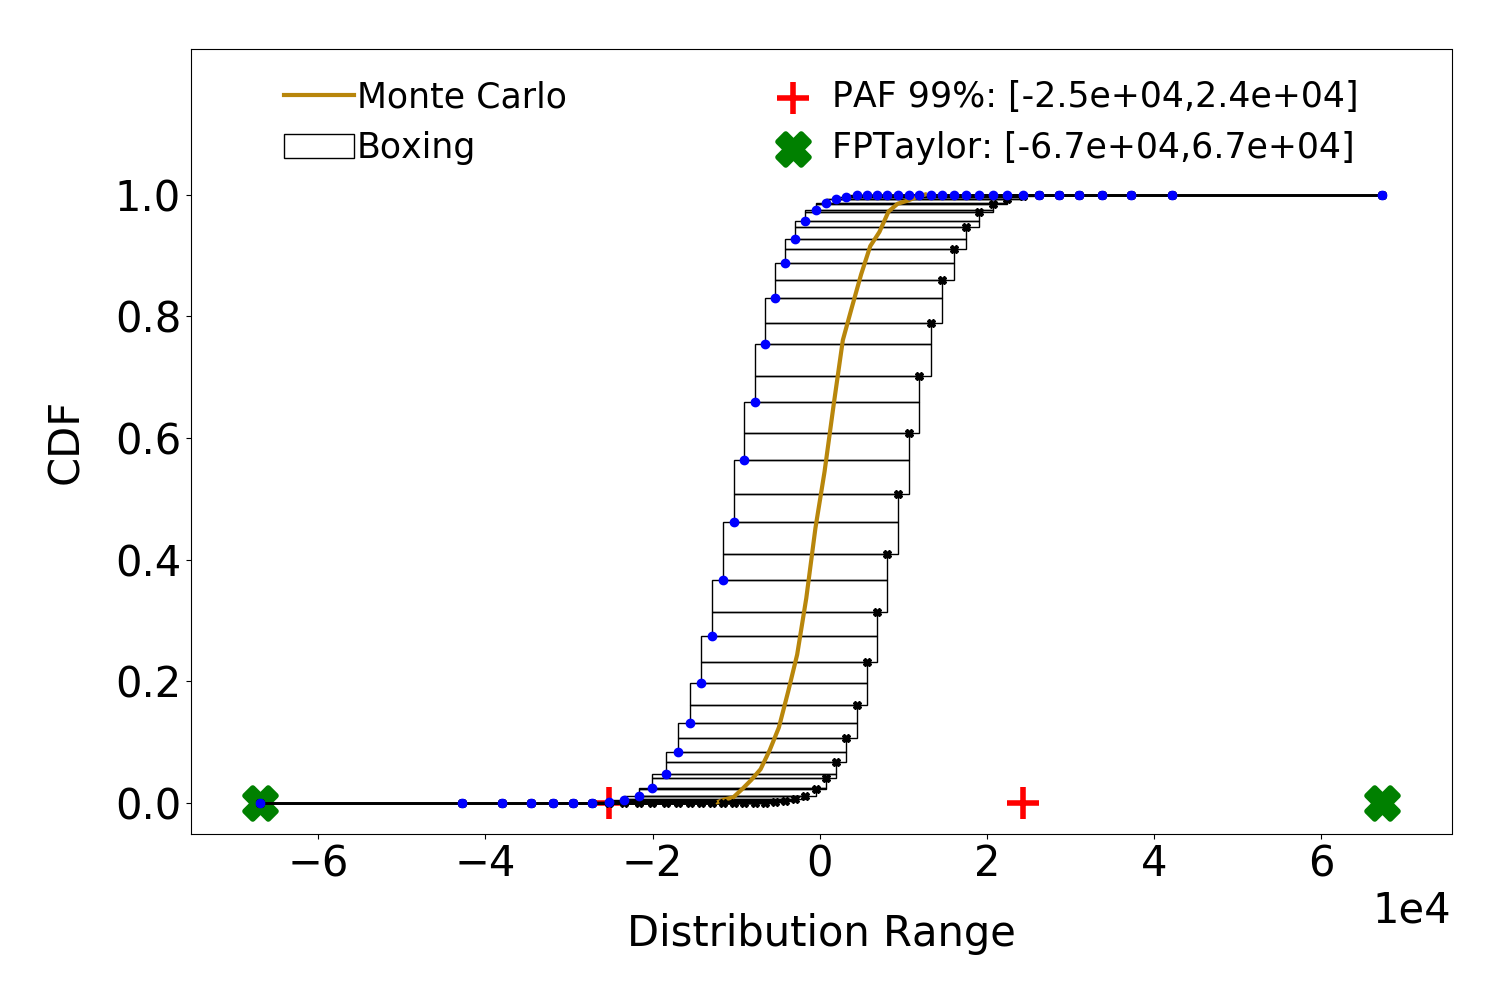
\includegraphics[width=0.5\textwidth]{pics/traincars3_gaussian_range_CDF.png}
		&
		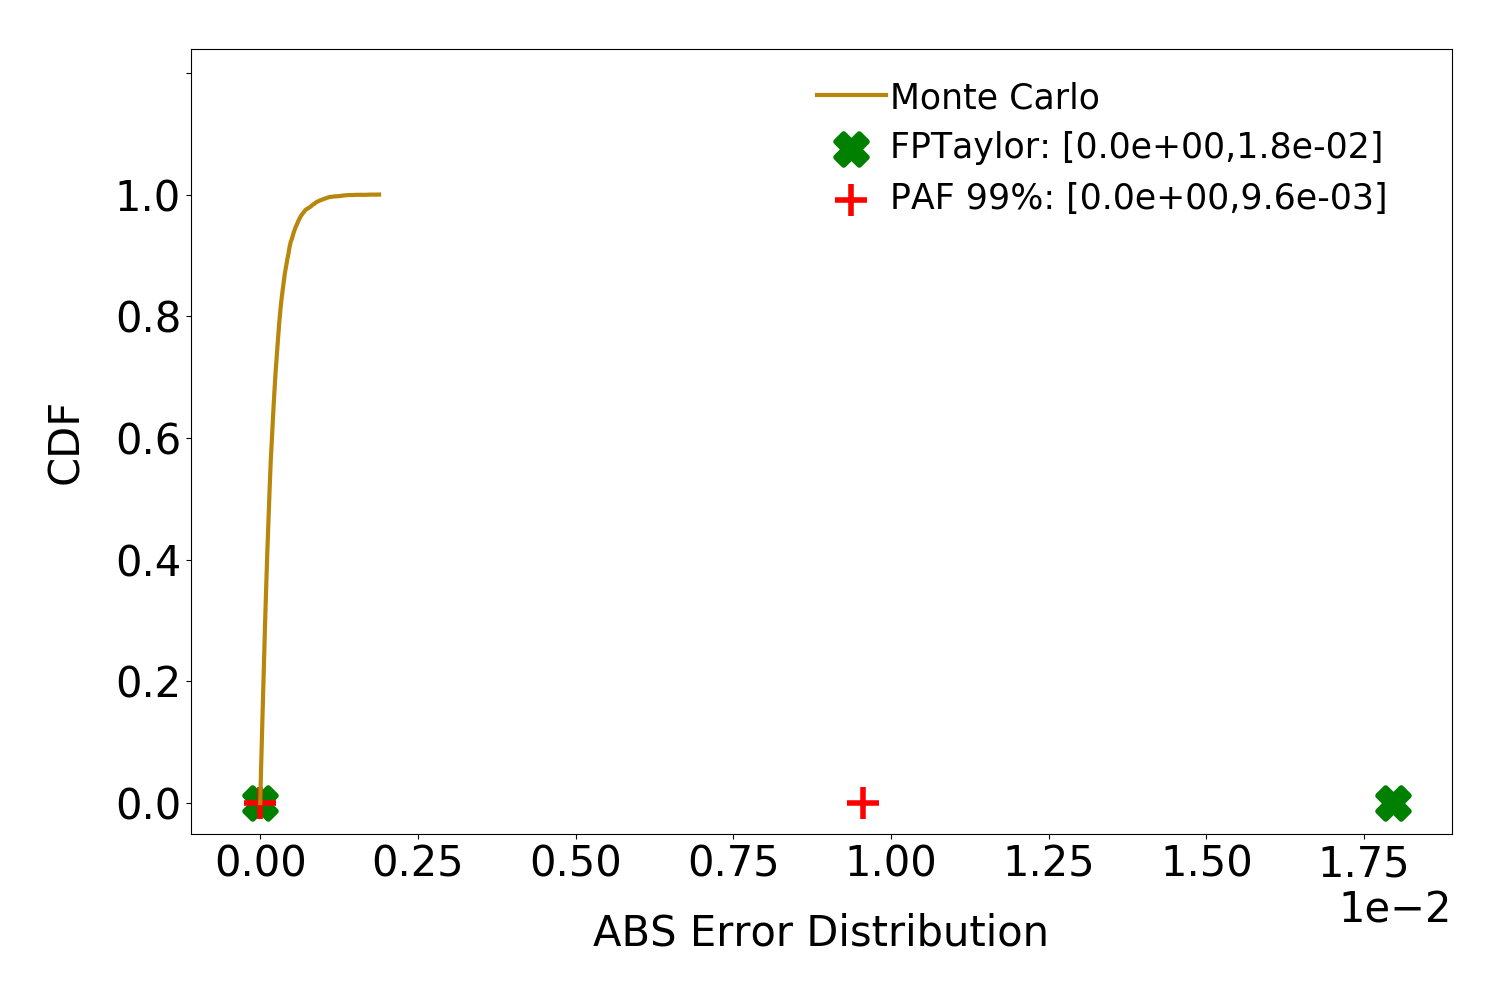
\includegraphics[width=0.5\textwidth]{pics/traincars3_gaussian_abs_error_CDF.png}
		\\
		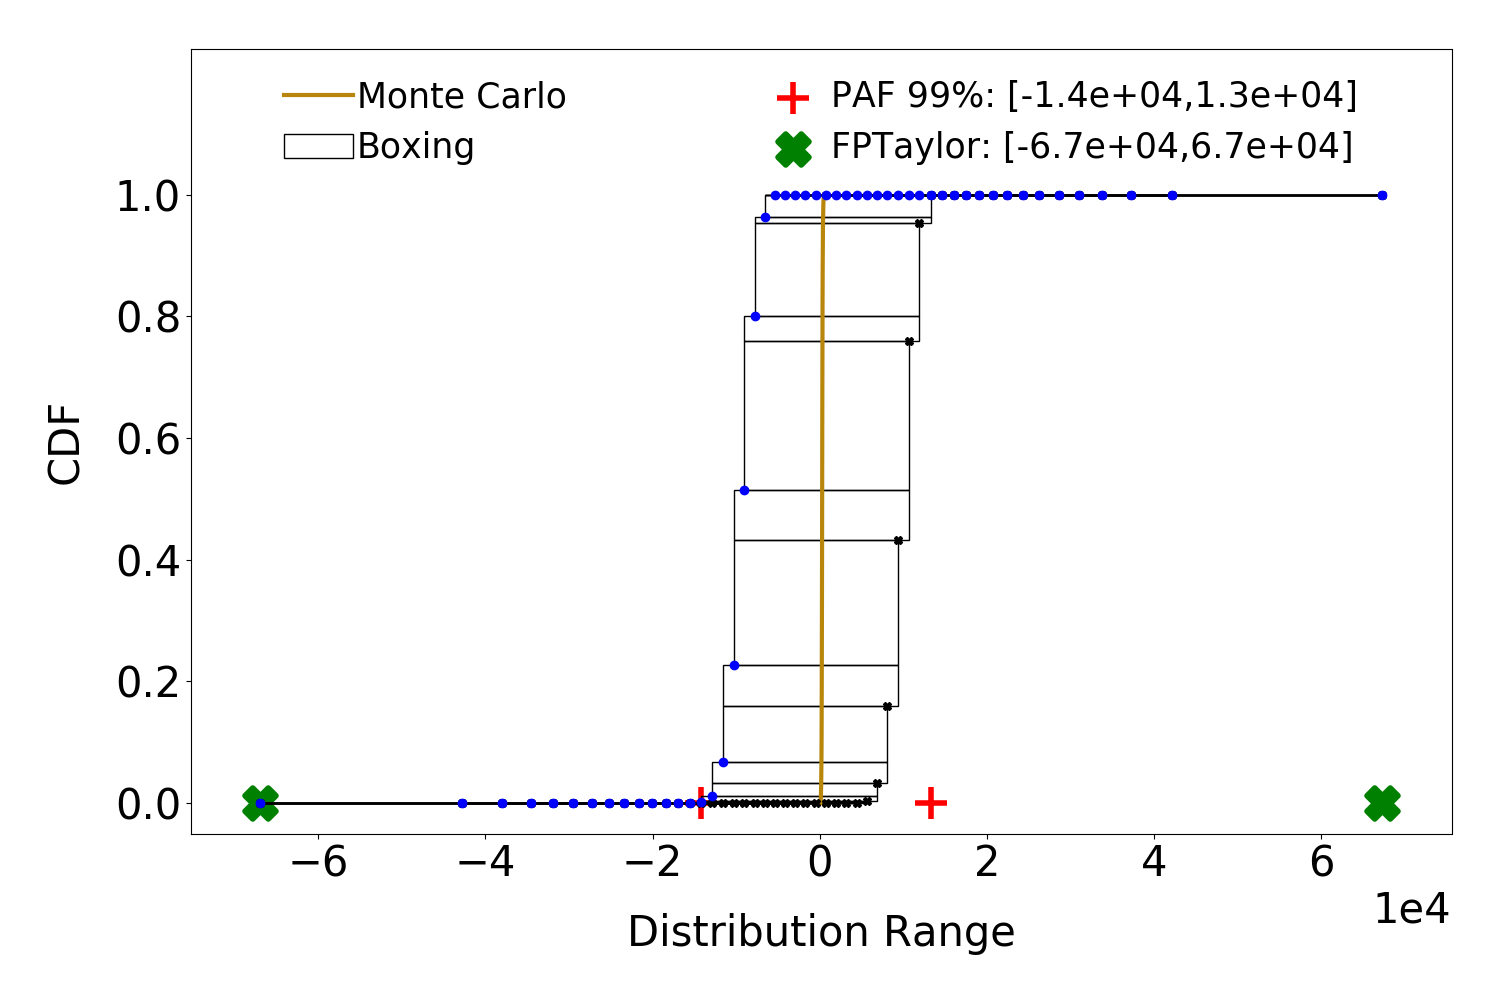
\includegraphics[width=0.5\textwidth]{pics/traincars3_exp_range_CDF.png}
		&
		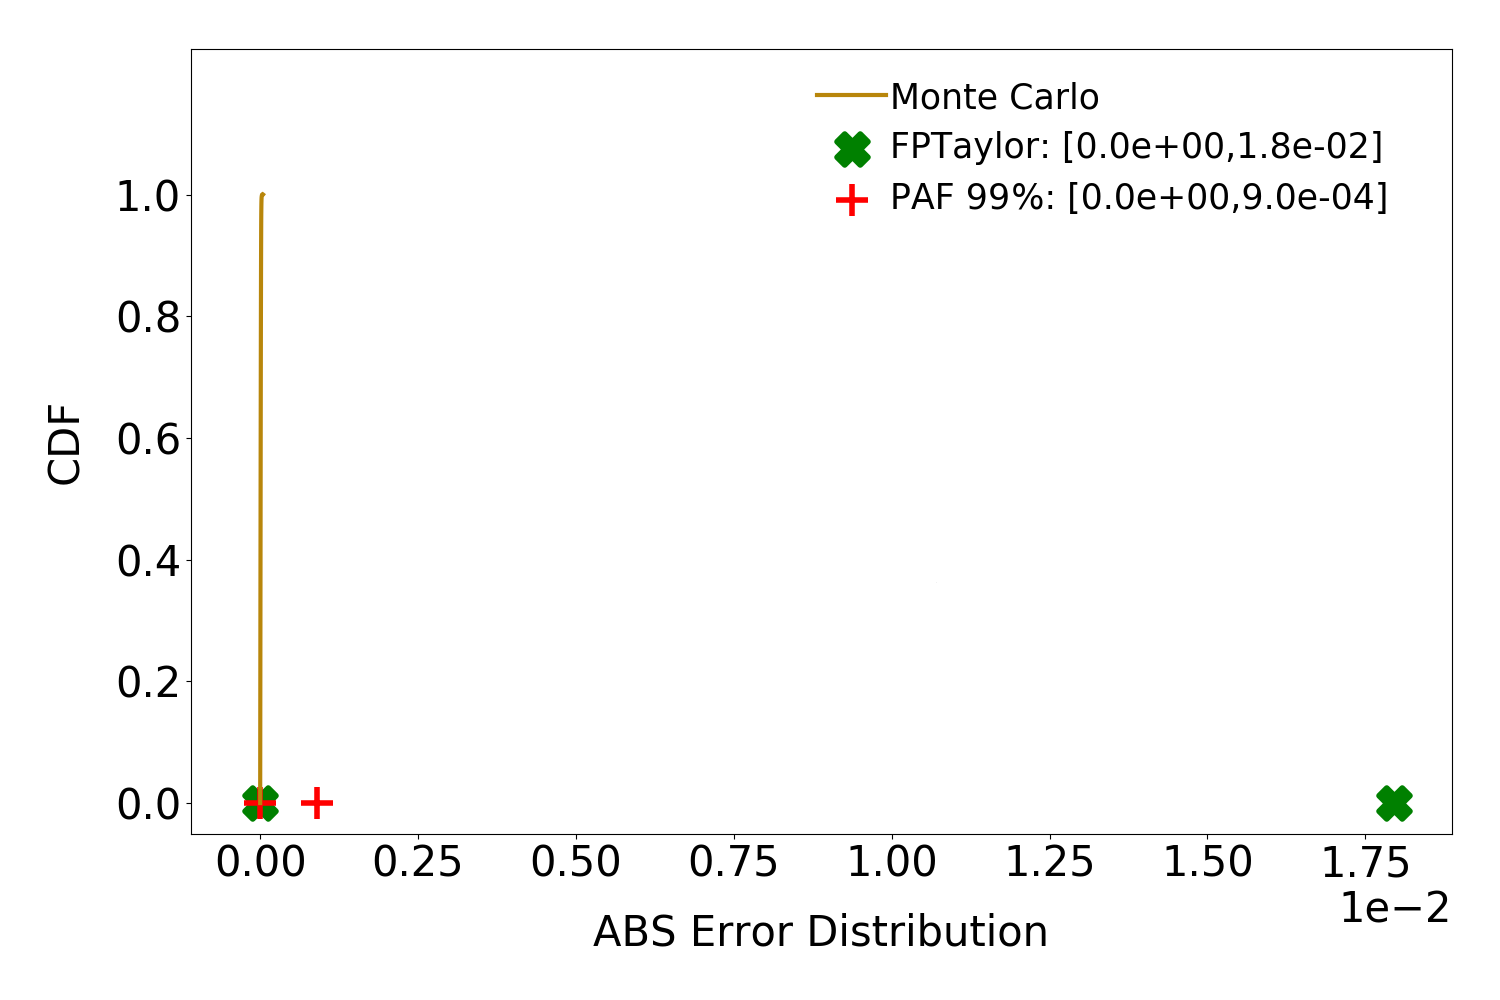
\includegraphics[width=0.5\textwidth]{pics/traincars3_exp_abs_error_CDF.png}
	\end{tabular}
	\caption{CDFs of the range (left) and error (right) distributions for the benchmark \emph{train3} for uniform (top), normal (center), and exp (bottom).}
	\label{fig:range_error_traincar}
\end{figure}


In general, we see a gradual reduction of the errors transitioning from uniform to normal to exp.
%
When the input distributions are uniform, there is a significant chance of generating a roundoff error of the same order of magnitude as the worst-case error, because all the inputs, including the extrema, are equally likely.
%
The standard normal distribution concentrates more than 99\% of probability mass in the interval $[-3, 3]$, thus resulting in the \emph{long tail} phenomenon, where less than 0.5\% of mass spreads in the interval $[3, \infty]$.\todo[inline]{Fred: is the input range is [20,20000] do you take the standard normal centred around the mid point? the leftmost point? around zero? Same question for exp.}
%
When the normal distribution gets truncated in a neighborhood of zero (e.g., $[0,1]$ for \emph{bsplines} and \emph{filters}) nothing changes with respect to the uniform case --- there is still a high chance of committing errors close to the worst-case.
%
However, when the normal distribution gets truncated in a wider range (e.g., $[-100, 100]$ for \emph{trids}) and we do have long tails, then the outliers causing large errors are very rare events, not included in the 99\% confidence interval.
%
The exponential distribution further compresses the 99\% probability mass in the tiny interval $[-0.01, 0.01]$, so the long tails effect is common among all the benchmarks. 
%
%Indeed, it suffices to have the interval $[-1, 1]$ to have already the \emph{long tails} effect.
%
%The only exception is \emph{bspline0}.
%
%For this benchmark, at \emph{any} intermediate computation, the probability mass associated to the extrema of the distribution is always significant. 
%
%There is then an hight chance of committing rounding errors close to the worst-case for all three input distributions.
%
%Please note for all the benchmarks the 100\% error is always equal to the uniform case.
%
%This means worst-case errors are not rare events for all three input distributions.
%
%Similar argument holds for \emph{bplines}, \emph{filters}, and \emph{sqrt} benchmarks in case of uniform and normal distributions. 

%The input distributions are truncated in a neighbor of zero (e.g. $[0, 1]$ for \emph{bsplines}, and $[-2, 2]$ for \emph{filters}). Near zero, the extrema of a normal distribution are still significant. In other words, sampling close to $1$, $-2$ or $2$ in case of normal input is not a rare event.
%

%When the input is exponentially distributed, the error bounds are further reduces compared to the normal case.
%
%The exponential distribution shrinks most of the probability mass (more than 99\%) in a tiny neighbor around zero. Indeed, between $-0.01$ and $0.01$ there is more than 99\% of the distribution.
%
%The error bounds from \Tool, PrAn, and FPTaylor are almost always in the same order of magnitude.
%
The runtimes of \Tool vary between 10 minutes for small benchmarks, such as
\emph{bsplines}, to several hours for benchmarks with more than 30 operations,
such as \emph{trid4}; they are always less than two hours, except for
\emph{trids} with 11 hours and \emph{filters} with 6 hours.
%
The runtime of \Tool is usually dominated by Z3 invocations, and the long
runtimes are caused by numerous Z3 timeouts that the respective benchmarks
induce.
%
The runtimes of PrAn are comparable to \Tool since they are always less than
two hours, except for \emph{trids} with 3 hours, \emph{sqrt} with 3 hours, and
\emph{sine} with 11 hours.
%
Note that neither \Tool nor PrAn are memory intensive, and hence memory
consumption is not an issue.



To assess the quality of our rigorous (i.e., sound) results, we implement
Monte Carlo sampling to generate both roundoff error and output range
distributions.
%
The procedure consists of randomly sampling from the provided input
distributions, evaluating the floating-point computation in both the specified
and high-precision (e.g., double-precision) floating-point regimes to measure
the roundoff error, and finally partitioning the computed errors into bins to
get an approximation (i.e., histogram) of the PDF.
%
Of course, Monte Carlo sampling does not provide rigorous bounds, but is a
useful tool to assess how far the rigorous bounds computed statically by \Tool
are from an empirical measure of the error.


Fig.\ref{fig:range_error_traincar} shows the effects of the input distributions
on the output and roundoff error ranges of the \emph{traincars3} benchmark.
%
In the error graphs (right column), we show the Monte Carlo sampling evaluation
(yellow line) together with the error bounds from \Tool with 99\% confidence
interval (red plus symbol) and FPTaylor's worst-case bounds (green crossmark). 
%
In the range graphs (left column), we also plot \Tool's p-box
over-approximations.
%
We can observe that in the case of uniform inputs the computed p-boxes overlap
at the extrema of the output range.
%
This phenomenon makes it impossible to distinguish between 99\% and 100\%
confidence intervals, and hence as expected the bound reported by \Tool is
almost identical to FPTaylor's.
%
This is not the case for normal and exponential distributions, where we can
observe the long tail phenomenon, and \Tool can significantly improve both the
output range and error bounds over FPTaylor.
%
%Also, we can see how the bounds from FPTaylor, both for the range and for the error, are always identical no matter the input distribution.
%
Hence, we again illustrate how pessimistic the bounds from worst-case tools can be when the information about the input distributions
is not taken into account.
%
%The empirical error has the shape of a curve in the uniform case, but becomes similar to a straight line for the exponential distribution. 
%
Finally, the graphs illustrate how the rigorous p-boxes and error bounds from
\Tool follow their respective empirical estimations, showing that \Tool adjusts
them based on the shape of the input distribution.

